\subsection{High-contrast diffusion and spatial bit placement}
\label{sec:revision-highcontrast}
We next use $-\nabla\cdot(\alpha\nabla u)=f$ on the same $16^2$ grid,
where $\alpha=0.01$ inside $(x-0.7)^2+(y-0.3)^2\le0.05$ and
$\alpha=1$ elsewhere. Harmonic face conductivities, including the
Dirichlet boundary faces, define the symmetric positive definite operator.
The low-conductivity region is separated from the source hotspot, so the
compression objective accounts for spatial response as well as source scale.
Using the independent hotspot source of Section~\ref{sec:revision-elliptic2d}
and $7$ bits per cell, we retain all
$14$ prescribed codecs and $30\,000$ paired source vectors. At length
$32$, the full-energy rule changes two precision blocks relative to Source
placement: it moves the extra-bit strip from $x\approx0.06,0.12$ toward
the low-conductivity region at $x\approx0.76,0.82$
(Figure~\ref{fig:revision-highcontrast-maps}). This reduces measured RMS by 19.97\%
(paired $95\%$ interval $[19.57,20.37]\%$); at length $128$,
the reduction is 11.25\% ($[10.34,12.17]\%$).
Table~\ref{tab:revision-highcontrast} gives the contiguous results;
both layouts and coincident maps remain in the package. The nominal intervals
contain 13 of $14$ population RMS predictions, with maximum
discrepancy 0.51\%. We also solve $100$ paired sources per codec
by Jacobi-preconditioned conjugate gradients at tolerance $10^{-11}$.
Since $A\succeq0.01A_{\rm Poisson}$, the preceding residual certificate
uses $0.01\lambda_{\min}(A_{\rm Poisson})$; its largest relative bound is
$8.4\times10^{-9}$, while PCG and direct-solve energy values agree within
$4.7\times10^{-11}$ relatively.

\begin{figure}[tb]
\centering
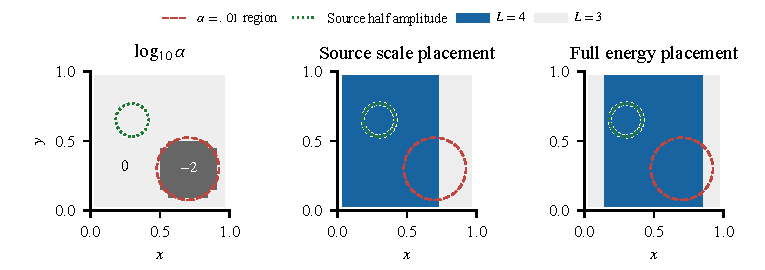
\includegraphics[width=\textwidth]{revision/experiments/highcontrast_precision_maps.pdf}
\caption{The prescribed diffusion coefficient and two length-$32$ contiguous
precision maps. The red disk marks the low-conductivity region; the green
outline is the half-amplitude source contour. Both maps have six blue
$L=4$ blocks and two gray $L=3$ blocks at the same storage cost.}
\label{fig:revision-highcontrast-maps}
\end{figure}

\begin{table}[tb]
\centering
\caption{High-contrast diffusion, $16^2$ sources and exactly $1792$ payload
bits. All entries use contiguous blocks; relative energy RMS is in percent.}
\label{tab:revision-highcontrast}
\begingroup\footnotesize\setlength{\tabcolsep}{5pt}
\begin{tabular}{rlrrr}
\toprule
$|B|$ & Placement & Exact & Ind. & MC $95\%$ interval\\
\midrule
8 & Uniform & 3.213 & 3.159 & [3.202,3.243] \\
32 & Uniform & 4.060 & 3.845 & [4.039,4.103] \\
32 & Source & 3.887 & 3.735 & [3.870,3.925] \\
32 & Energy & 3.114 & 3.005 & [3.099,3.139] \\
128 & Source & 8.948 & 7.993 & [8.817,8.991] \\
128 & Energy & 7.916 & 6.761 & [7.824,7.978] \\
\bottomrule
\end{tabular}\endgroup
\end{table}
